\chapter{Анализ предметной области}
\section{Основные понятия корпусной лингвистики}

Корпусная лингвистика~---~раздел компьютерной лингвистики, занимающийся разработкой общих принципов построения и использования лингвистических корпусов (корпусов текстов) с применением компьютерных технологий. Под лингвистическим, или языковым, корпусом текстов понимается большой, представленный в машиночитаемом виде, унифицированный, структурированный, размеченный, филологически компетентный массив языковых данных, предназначенный для решения конкретных лингвистических задач~\cite{Zaharov}. Существуют также альтернативные определения понятия <<языковой корпус>>. Например, корпус текстов – вид корпуса данных, единицами которого являются тексты или их достаточно значительные фрагменты, включающие, например, какие-то полные фрагменты макроструктуры текстов определённой проблемной области~\cite{Grudeva}.

В современной компьютерной лингвистике понятие <<корпус текстов>> подразумевает также специализированную поисковую систему, включающую программные средства для поиска данных в корпусе, получения статистической информации и предоставления пользователю результатов в удобной форме, называемую корпусным менеджером~\cite{Zaharov}.

В соответствии с описанным выше, современный корпус предполагает также наличие аннотации или разметки. Аннотация~---~это приписанная всем единицам выбранного уровня (текст, предложение, словоформа и т.~д.) соответствующая лингвистическая информация. При этом аннотирование может быть представлено одновременно для различных уровней~\cite{Kopotev}.

Поиск по слову в корпусе позволяет построить конкорданс~---~список всех словоупотреблений данного слова в контексте с указанием источников~\cite{Zaharov}. Таким образом корпусы могут быть использованы для получения разнообразных справок и статистических данных о языковых я речевых единицах. В более широком смысле конкорданс~---~особый тип словаря, в котором каждое слово или понятие сопровождается минимальным контекстом и всеми случаями употребления в некотором тексте. Иногда конкроданс также определяют как словарь сочетаемости языковых единиц, словарь контекстов~\cite{concordanceDominican}. Конкордансы могут быть использованы в лингвистике в следующих целях~\cite{Dobrinina}:
\begin{itemize}
	\item сравнение различных использований одного слова;
	\item анализ частотности слов и словосочетаний;
	\item поиск и исследование фраз и идиом;
	\item поиск перевода, например, терминологии;
	\item анализ ключевых слов.
\end{itemize}
Конкордансы также могут использоваться для анализа творчества отдельных писателей~\cite{Kalinkin,Vasilev} и обучения иностранным языкам~\cite{Nagel}.

Тезаурус в современной лингвистике~---~особая разновидность словарей общей или специальной лексики, в которых указаны семантические отношения (синонимы, антонимы, паронимы, гипонимы, гиперонимы и т.~п.) между лексическими единицами~\cite{Kopotev}.

Еще одним понятием корпусной лингвистики является онтология. Несмотря на множество определений онтологии многие авторы соглашаются в наборе основных компонентов онтологии: классы или понятия; атрибуты (свойства); экземпляры (отдельные индивиды), отношения между классами или экземплярами; аксиомы онтологии. Исходя из этого формально можно определить онтологию следующим образом:
\begin{equation*}
	O = <C,\ E,\ A_t,\ R,\ A>,
\end{equation*}
где $C$~---~понятия (классы) онтологии, $E$~---~экземпляры онтологии, $A_t$~---~атрибуты понятий и экземпляров онтологии, $R$~---~отношения между понятиями, $A$~---~аксиомы онтологии.

Таким образом объектом корпусной лингвистики является корпус текстов, который, с одной стороны, представляет собой исходный материал для корпусной лингвистики и других разделов лингвистики; с другой стороны, является результатом деятельности корпусной лингвистики~\cite{Zaharov}.

Предметом корпусной лингвистики являются теоретические основы и практические механизмы создания и использования представительных массивов языковых данных, предназначенных для лингвистических исследований в интересах широкого круга пользователей~\cite{Zaharov}.

\section{История развития корпусной лингвистики}

Истоки корпусной лингвистики, ее приемов и методов прослеживаются начиная с момента создания грамматики санскрита Панини около V в. до н. э., представлявшей собой систематизацию уже существовавшей в ритуальных текстах грамматики~\cite{Voloshina,Kopotev}. 

В дальнейшем основным направлением развития корпусной лингвистики стало составление конкордансов основанных на Библии. Первым из известных на данный момент конкордансов является связанный с именем Антония Падуанского <<Concordantiae morales sacrae scripturae>> (<<Нравственная конкорданция Священного Писания>>), появившийся в начале XIII века~\cite{handbook,Kopotev}.

Следующим этапом развития корпусной лингвистики связан с развитием лексикографии и создания словарей языков в XVIII--XIX веках. Появившиеся в это время словари и грамматики составлялись на основе крупных картотек или произведений признанных авторов~\cite{Kopotev}. Так, например, Словарь живого великорусского языка В. И. Даля основан на материалах как предшествующих ему словарей, так и на самостоятельно подобранных, при этом слова приводятся с примерами использования, что близко по смыслу к конкордансу, построенному на основе существовавших на тот момент литературного и народного языков~\cite{Dal,Kopotev}. В английском языке словарями, основанными на обработке и выборке примеров употребления из существующих произведений литературы, принято считать <<Американский словарь английского языка>> (<<An American dictionary of the English language>>) Н. Вебстера~\cite{Webster} и толковый словарь английского языка (<<Dictionary of the English language>>) С. Джонсона~\cite{Johnson}. Г. Пауль для составления немецкой грамматики (<<Deutsche Grammatik>>~\cite{Paul}) использовал произведения немецких <<классиков>> для иллюстрации своих утверждений~\cite{Zaharov}.

В конце XIX~--~начале XX века начинают появляться корпусы специально созданные для лингвистических исследований или решения практических задач. Одной из таких задач являлся подсчет частотности языковых единиц. Первым словарем такого рода стал <<Частотный словарь немецкого языка>> (<<Häufigkeitswörterbuch der deutschen Sprache>>~\cite{Kaeding}). Данный словарь был подготовлен на основе корпуса содержащего одиннадцать миллионов словоупотреблений~\cite{Kopotev}. 

В 1909 году был опубликован первый том <<A Modern English Grammar on Historical Principles. Part I. Sounds and spellings>>~\cite{Jespersen} датского ученого Отто Есперсена. Основной идеей труда Есперсена был переход от нормативных грамматик к дескриптивным, т.~е. анализирующим и описывающим использование языка в живой речи. Для подкрепления изложенных в грамматике тезисов Есперсен специально подбирал источники примеров, общее изложение которых заняло 40 страниц и представляет собой прообраз современного репрезентативного корпуса~\cite{Kopotev}. В связи с необходимостью ручного подбора и обработки выход всех семи томов данной работы затянулся на 40 лет.

\section{Классификация корпусов}

В зависимости от цели разработки корпусы могут классифицироваться самым разным образом. Выделенные в~\cite{Zaharov} типы классификаций представлены в таблице~\ref{tab:classification_1}.

\begin{table}[H]
	\centering
	\caption{Виды классификаций корпусов}
	\begin{tabular}{|l|l|}
		\hline 
		Признак классификации & Типы корпусов \\
		\hline
		\multirow{3}{*}{Тип языковых данных} & Письменные \\\cline{2-2} 
		 & Устные \\\cline{2-2}
		 & Смешанные \\\hline
		\multirow{3}{*}{<<Параллельность>>} & Одноязычные \\\cline{2-2}
		 & Двуязычные \\\cline{2-2}
		 & Многоязычные \\\hline
		 \multirow{5}{*}{<<Литературность>>} & Литературные \\\cline{2-2}
		 & Диалектные \\\cline{2-2}
		 & Разговорные \\\cline{2-2}
		 & Терминологические \\\cline{2-2}
		 & Смешанные \\\hline
		\multirow{2}{*}{Цель} & Многоцелевые \\\cline{2-2}
		 & Специализированные \\\hline
		\multirow{4}{*}{Жанр}&Литературные\\\cline{2-2}
		 &Фольклорные\\\cline{2-2}
		 &Драматургические\\\cline{2-2}
		 &Публицистические\\\hline
		\multirow{3}{*}{Доступность}&Свободно доступные\\\cline{2-2}
		 &Коммерческие\\\cline{2-2}
		 &Закрытые\\\hline
		\multirow{2}{*}{Назначение}&Исследовательские\\\cline{2-2}
		 &Иллюстративные\\\hline
		\multirow{2}{*}{Динамичность}&Динамические (мониторные)\\\cline{2-2}
		 &Статические\\\hline
		\multirow{2}{*}{Разметка}&Размеченные\\\cline{2-2}
		 &Неразмеченные\\\hline
		\multirow{2}{*}{Объем текстов}&Полнотекстовые\\\cline{2-2}
		&<<Фрагментнотекстовые>>\\\hline
	\end{tabular}
	\label{tab:classification_1}
\end{table}

По типу языковых данных корпусы делятся на письменные, устные, смешанные. В письменных корпусах (Брауновский корпус~\cite{bibid}, корпус Ланкастер-Осло-Берген~\cite{bibid}) устная речь не представлена, в устных представлена только устная, к смешанным обычно относят национальные корпусы, представляющие язык в определенный период времени (Национальный корпус русского языка~\cite{bibid}, Британский национальный корпус~\cite{bibid})~\cite{Zaharov}.

По критерию параллельности корпусы делятся на одноязычные, двуязычные и многоязычные. В одноязычных противопоставляются диалекты, варианты языка. Двуязычные и многоязычные корпусы объединяют тексты одной и той же тематической области, независимо написанные на двух или нескольких языках. Зачастую основой таких корпусов также является множество текстов-оригиналов на каком-либо исходном языке и текстов-переводов исходных текстов на один или несколько других языков~\cite{Zaharov}. В~\cite{Kopotev} двуязычные относят к многоязычным, среди которых дополнительно выделяют выровненные (параллельные), т.~e. связанные на уровне абзацев или предложений, и невыровненные. В случае использования параллельных корпусов построенных на основе текстов-переводов возможно автоматическое выравнивание на этапе построения таких текстов~\cite{Baranov,Zubov}.

По критерию <<литературности>> выделяются литературные, диалектные, разговорные и терминологические корпусы~\cite{Zaharov}.

По цели создания корпусы делятся на многоцелевые и специализированные. Многоцелевые корпусы содержат тексты различных жанров (к ним же относятся национальные корпусы), тогда как специализированные корпусы могут ограничиваться одним жанром или группой жанров~\cite{Zaharov}.

Корпусы текстов могут быть классифицированы по жанрам и подразделяться на литературные, фольклорные, драматургические, публицистические и др. Примерами публицистического корпусы могут служить Компьютерный корпус текстов русских газет конца ХХ-ого века~\cite{bibid} и корпус
политических метафор~\cite{bibid}.

По доступности корпусы подразделяются на свободно доступные, коммерческие и закрытые. Стоит отметить, что закрытые корпусы предназначены для специфических задач и потому не представлены в открытом доступе~\cite{Zaharov}. Иногда дополнительно выделяют также доступные по академической лицензии для использования в научной некоммерческой деятельности~\cite{Kopotev}.

По назначению выделяют исследовательские и иллюстративные корпусы. Исследовательские корпусы создаются с целью с целью изучения различных аспектов функционирования языка. Поскольку этот тип корпусов ориентирован на широкий класс лингвистических задач, что требует при построении таких корпусов использовать специальные способы обеспечения репрезентативности. Такие корпусы содержат как правило от десятков до сотен миллионов словоупотреблений. Иллюстративные корпусы создаются после проведения исследования с целью подтверждения и обоснования полученных результатов~\cite{Zaharov}.  

Критерий <<динамичность>> подразделяет корпусы на динамические и статические. Статические корпусы содержат корпусы небольшого временного промежутка~\cite{Zubov}. Типичными представителями такого рода корпусов являются авторские корпусы~---~коллекции текстов писателей~\cite{Zaharov}. Динамические корпусы служат для выявления функционирования языковых феноменов на временной шкале~---~например, изменения значения слов, частоты использования тех или иных синтаксических конструкций~\cite{Baranov}.

По критерию <<разметка>> корпусы делятся на размеченные и неразмеченные. В размеченном корпусе словам или предложениям присваиваются метки (тэги) в соответствии с характером разметки: морфологические, синтаксические, семантические, просодические и другие~\cite{Zaharov}.

По критерию <<объем текстов>> выделяются полнотекстовые и так называемые фрагментотекстовые. Брауновский корпус и корпус Ланкастер-Осло-Берген были строго ограничены числом словоупотреблений, поэтому являются фрагментотекстовыми. К полнотекстовым относятся как правило корпусы определенного автора, а также корпусы коротких текстов, например, корпусы газетных заголовков~\cite{Zaharov}.

В~\cite{Grudeva} выделяются дополнительно критерии общности и хронологического аспекта. По критерию <<общности>> корпусы разделяют на коллекции текстов принадлежащие одному писателю и различным. По критерию хронологического аспекта корпусы делят на синхронические и диахронические, которые в сущности совпадают с ранее описанными динамическими и статическими типами.

Дополнительно среди фрагментнотекстовых корпусов выделяют конкордансные и корпусы n-грамм~\cite{Kopotev}.

Таким образом в данной работе рассматриваются письменные, выровненные, многоязычные, научно-технические, свободно доступные, исследовательские, статические, неразмеченные, фрагментнотекстовые корпусы.

\section{Репрезентативность корпуса}

Представительность корпуса получила название репрезентативности, а соотношение отдельных его частей (по разным характеристикам)~---~сбалансированности~\cite{ZaharovSpec}. В настоящее время считается, что объем общеязыкового корпуса должен составлять не менее 100 миллионов словоупотреблений. Имеются разные походы к определению репрезентативности. Одним из способов является измерение насыщенности частотного словаря (относительные частоты лексем не меняются или меняются незначительно)~\cite{Zaharov}.

Поскольку корпус представляет собой уменьшенную модель языка для специальных целей (то есть языка технических текстов), под его сбалансированностью понимается необходимое и достаточное пропорциональное представление в корпусе различных текстов данной проблемной области или данного типа, т.~е. способность отражать все свойства изучаемого подъязыка~\cite{ZaharovSpec}.

Когда говорят о сбалансированном корпусе, то понимают также сбалансированность его по возможностям: правильно налаженный корпус предполагает модель программно-лингвистического инструмента, поддающуюся настройке и регулированию~\cite{ZaharovSpec}.

\section{Виды разметок}

Джеффри Лич приводит следующие принципы, которым должна подчиняться разметка общедоступного корпуса~\cite{Leech1997}:
\begin{itemize}
	\item разметка должна основываться на доступной для пользователя в виде руководства или инструкции схеме анализа, в которой должно быть мотивированно введение каждого параметра;
	\item разметка общедоступного корпуса должна опираться на общеизвестную систему правил и классификаций;
	\item должно быть ясно кто и как разрабатывает схему аннотации и каковы ограничения, например юридические или технические, при использовании корпусом~\cite{Kopotev}.
\end{itemize}

В соответствии с~\cite{Lesnikov,Zaharov,Kopotev,trudy2019} выделяются следующие типы разметки:
\begin{itemize}
	\item анафорическая;
	\item дискурсная;
	\item жанровая;
	\item издательская;
	\item метатекстовая;
	\item морфологическая;
	\item синтаксическая;
	\item семантическая;
	\item служебная;
	\item структурная;
	\item терминологическая.
\end{itemize}

Анафорическая разметка необходима для установления референтных связей, т.~е. соотнесение включенных в речь имен, именных выражений или их эквивалентов к реальным объектам. В связи с широким распространением в технических текстах аббревиатур и других референций вместо определенного термина (например, <<аппарат>>, <<ЛА>> вместо <<летательный аппарат>>), при использовании средств машинной разметки таких текстов необходимо учесть все возможные референции встречающихся терминов, чтобы итоговая статистическая картина частотности употребления термина не была искаженной.

Дискурсная разметка зачастую реализуется для текстов художественного и разговорного стилей, речевых корпусов. Поскольку научно-техническим текстам не свойственно присутствие дискурсных единиц~\cite{bogdanova2014}, реализация данной разметки для корпусов таких текстов не является необходимой.

Жанровая разметка для корпуса научно-технических текстов реализуется при отборе текстов для наполнения корпуса. 

Издательская разметка отражает особенности форматирования текста, которые могут быть использованы при реализации других видов разметок. 

Метатекстовая (экстралингвистическая) подразумевает под собой добавление к тексту внетекстовых характеристик: авторов, год, издательство, журнал, жанр и другие особенности текста или обстоятельства его создания. Выделяют два класса факторов влияющих на язык текстов и описываемых метатекстовой разметкой~\cite{Zaharov}:
\begin{itemize}
	\item внешние, внеязыковые факторы (E~---~external);
	\item внутренние, относящие к внешним признакам текста (I~---~internal).
\end{itemize}

Дж. Синклер выделяет три группы E-факторов~\cite{sinclair1996preliminary}:
\begin{itemize}
	\item E1 (origin)~---~факторы, относящиеся к созданию текста автором;
	\item E2 (state)~---~факторы относящиеся к внешним признакам текста;
	\item E3 (aims)~---~факторы, относящиеся к причинам создания текста и его влиянию на аудиторию.
\end{itemize}
И две группы I-факторов:
\begin{itemize}
	\item I1 (topic)~---~предметная область текста;
	\item I2 (style)~---~стилистические особенности текста (стиль, жанр).
\end{itemize}

Морфологическая разметка включает в себя: лемму (начальную форму слова), признак части речи, признаки грамматических категорий в зависимости от части речи. Данный тип разметки~---~основной и реализован в большинстве корпусов, а также является основой для дальнейших форм анализа~---~синтаксического и семантического. Кроме того в современных корпусах, этот тип разметки может быть реализован автоматически~\cite{Zaharov}.

В корпусной лингвистике синтаксическая разметка основана на грамматике зависимостей~\cite{Zaharov,Kopotev}. Тексты, получившие синтаксическую разметку известны в англоязычной литературе как treebanks~\cite{abeeille2003treebanks}. Пример визуализации синтаксических зависимостей, отображаемых синтаксической разметкой, представлен на рисунке~\ref{fig:syntax_annotation}.

\begin{figure}[H]
	\centering
	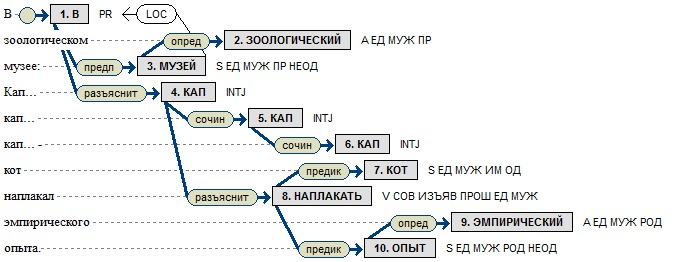
\includegraphics[width=0.9\linewidth]{images/syntax_annotation.png}
	\caption{Визуализация синтаксических зависимостей в НКРЯ}
	\label{fig:syntax_annotation}
\end{figure}

Семантическая разметка состоит в приписывании единицам текста одной или нескольких семантических категорий. Семантические тэги чаще всего обозначают семантические категории, к которым относится данное слово или словосочетание, и более узкие подкатегории, специфицирующие его значение. Семантическая разметка корпусов предусматривает определение значения слов, разрешение омонимии и категоризацию слов, выделение тематических классов и т.~д.~\cite{Zaharov}.

При этом к семантической разметке относят и категоризацию семантических ролей~\cite{Kopotev}. Семантические роли под названием <<глубинные падежи>> впервые выделены и описаны Ч. Филлмором~\cite{fillmore1968case}. Семантическая роль имени при данном предикате является частью семантики этого предиката и отражает общие свойства участников определенных групп ситуаций. В данном определении предполагается, что предикатные (глагольные) лексемы описывают <<ситуации>>, а именные лексемы~---~<<участников>> этих ситуаций, которые называются аргументами предикатов. Состав и количество семантических ролей, выделяемых при том или ином описании, зависят от конкретной задачи и могут существенно различаться; в большинстве случаев достаточно сравнительно небольшого набора из двух - трех десятков ролей.~\cite{plungian2003obshtaya}.

Служебная разметка используется для приписывания текстам информации о стиле и целевой аудитории текстов в корпусе. Реализация этого типа разметки в параллельном корпусе технических текстов нецелесообразна в силу отсутствия значимых различий в стиле текстов и целевой аудитории.

Структурная разметка маркирует главы, абзацы, предложения и словоформы~\cite{kibrik2019introduction}. Для проведения структурной разметки необходимо обосновать процедуру сегментации текста, т.~е. его разбиение на необходимые и достаточные сегменты, релевантные для его компьютерной обработки, позволяющие пользователю определить лексические, грамматические и другие свойства изучаемых лингвистических единиц~\cite{gorban2021structural}. 

Терминологическая разметка предназначена для фиксации в тексте имен понятий предметной области~\cite{zagorulko2013software}. Терминологическая разметка позволяет не только фиксировать присутствие определенных терминов в тексте, но и~\cite{zagorulko2012system}:
\begin{itemize}
	\item определять максимальный текстовый фрагмент, представляющий сущность. При этом остается возможность указывать и вложенные фрагменты, представляющие самостоятельные сущности;
	\item сопоставлять аннотацию самой сущности, а не всей синтаксической 	группе, в которую она входит;
	\item  использовать при необходимости разрывные фрагменты, в том числе при перечислении с сочинительным сокращением.
\end{itemize} 

Исходя из приведенного анализа видов разметки система управления корпусными данными параллельных корпусов технических текстов должна реализовывать следующие виды разметки: анафорическую, метатекстовую, морфологическую, семантическую, синтаксическую, структурную и терминологическую. При этом как было отмечено выше, существует большое количество автоматических морфологических анализаторов.

\chapter{Обзор методов построения разметки текстов}
\section{Анафорическая разметка}

Как было отмечено выше, анафорическая разметка отвечает за установление референтных связей. Глобально выделяют два вида анафоры: именную, называемую также корефернтной или кореферетностью, и местоименную~\cite{sokolov2017razrabotka}. Пример именной анафоры был приведен выше. В случае местоименной анафоры анафор выражен местоимением.

Для автоматического разрешения анафоры (определения антецедента~---~выражения, к которому отсылает анафор) в настоящие время выделяют два подхода:
\begin{itemize}
	\item разрешение на основе правил~\cite{bogdanov2014anaphora,mitkovStateOfArt,carter1987interpreting,baldwin1997cogniac,azerkovich2019ispolzovanie,Ng2017MachineLF};
	\item разрешение на основе методов машинного обучения~\cite{inshakova2019razvitie,sokolov2017razrabotka,protopopova2014experience,eremeeva2018razreshenie,tolpegin2006algorithm,mitkovStateOfArt,Ng2017MachineLF}.
\end{itemize}

Как видно из приведенных источников, в современной русскоязычной среде преобладает подход с использованием машинного обучения, тогда как в англоязычных работах изначально рассматривался подход с использованием системы правил.

\subsection{Вычисление семантической близости}

В~\cite{azerkovich2019ispolzovanie} описывается сравнение различных метрик семантической близости, которая может быть использована как решающий критерий при выборе одного из множества антецедентов данного анафора. Семантическая близость вычислялась на основе  открытой части онтологии русского языка RuThes~\cite{lukashevich2011thesauri} и текстов корпуса RuCor~\cite{toldova2016russian}. В работе выделяются три класса метрик, в зависимости от принципа подсчета, на котором они основаны:
\begin{enumerate}
	\item метрики, основанные на длине пути $path(c_1, c_2)$ между вершинами онтологии $c_1$, $c_2$, соответствующими искомым сущностям~\cite{rada1989development}. В дальнейшем было предложено два метода нормализации:
	\begin{itemize}
		\item с учетом глубины онтологии $D$~\cite{wu1994verb}:
		\begin{equation}
			wp(c_1,\ c_2) = -ln\frac{path(c_1,\ c_2)}{2D}
		\end{equation}
		\item с учетом глубины узлов онтологии $depth(c_i)$~\cite{leacock1998combining}:
		\begin{equation}
			lc(c_1,\ c_2)=\frac{2depth(lca)}{depth(c_1)+depth(c_2)},
		\end{equation}
		где $lca$~---~наименьший общий предок узлов $c_1$ и $c_2$.
	\end{itemize}
	\item метрика, основанная на подсчете информационной содержательности, т.~е. частота встречаемости понятия, которая рассчитывается как вероятность его появления в корпусе текстов~\cite{resnik1995using}. Метод расчета семантической близости основанный на этой величине описан в~\cite{seco2004intrinsic} и использует информационную содержательность наименьшего общего предка вершин $c_1$ и $c_2$, соответствующих искомым сущностям:
	\begin{equation}
		res(c_1,\ c_2) = 1 - \frac{ln(hypo(lca)+1)}{ln(max_{wn})},
	\end{equation}
	где $lca$~---~наименьший общий предок, $hypo(n)$~---~число гипонимов узла, $max_{wn}$~---~число вершин в онтологии.
	\item метрика, основанная на расчете текстовых пересечений, предложенная в~\cite{lesk1986automatic}. Ее вычисление основано на количестве пересечений различной длины между текстами:
	\begin{equation}
		\label{eq:overlap}
		overlap(t_1,\ t_2) = \sum^{n}_{i=1} m^2,
	\end{equation}
	для $m$ $n$-словных пересечений между текстами $t_1$ и $t_2$. В статье~\cite{ponzetto2006exploiting} предлагается метод нормализации данной метрики с учетом длины сравниваемых текстов:
	\begin{equation}
		lesk(t_1,\ t_2)=th(\frac{overlap(t_1,\ t_2)}{length(t_1)+length(t_2)}),
	\end{equation} 
	где $overlap(t_1,\ t_2)$ определяется в соответствии с~\ref{eq:overlap}, а $length(t_i)$~---~длина фрагмента текста $t_i,\ i=\overline{1,2}$
\end{enumerate}

Приведенные в~\cite{azerkovich2019ispolzovanie} результаты сравнения указанных метрик, отражены в таблице~\ref{tab:compare_semantic_path}. Метрика lesk не могла быть подсчитана на данных из RuThes, поскольку глоссы в нем приведены лишь для очень небольшого числа сущностей~\cite{azerkovich2019ispolzovanie}.

\begin{table}[H]
	\centering
	\caption{Значения коэффициента корреляции метрик семантической близости с кореферентной разметкой}
	\begin{tabular}{|l|r|r|r|r|r|}
		\hline 
		Источник &\multicolumn{1}{c|}{\textit{path}} & \multicolumn{1}{c|}{\textit{wp}} & \multicolumn{1}{c|}{\textit{lc}} & \multicolumn{1}{c|}{\textit{res}} & \multicolumn{1}{c|}{\textit{lesk}} \\
		\hline
		RuThes & 0,56 & 0,51 & 0,59 & 0.30 & n/a \\\hline
	\end{tabular}
	\label{tab:compare_semantic_path}
\end{table}

\subsection{ABBYY Compreno}

Технология ABBYY Compreno описана в~\cite{bogdanov2014anaphora,zuev2013statistical,anisimovich2012syntactic}. Поскольку данная технология является проприентарной, достоверно неизвестно, какие именно механизмы используются для разрешения кореференции и анафоры.

Однако, исходя из текста статьи, можно сделать вывод, что для разрешения анафоры используется построенное семантическое дерево предложения, в которое дополнительно включаются связи, не принадлежащие исходному дереву. Кроме того, анафора заменяется антецедентом. Исходное семантическое дерево предложения: <<Мальчик дал девочке свое яблоко>>,~---~представлено на рисунке~\ref{fig:compreno_syntax_without}. 
\begin{figure}[H]
	\centering
	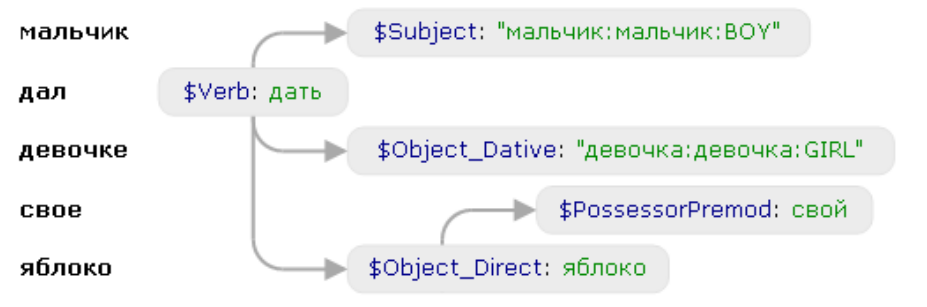
\includegraphics[width=0.9\linewidth]{images/compreno_syntax_without.png}
	\caption{Семантическое дерево, построенное системой Compreno}
	\label{fig:compreno_syntax_without}
\end{figure}

На рисунке~\ref{fig:compreno_syntax_with} представлено семантическое дерево с дополнительной связью от антецедента к анафору, при этом анафор заменен на антецедента.
\begin{figure}[H]
	\centering
	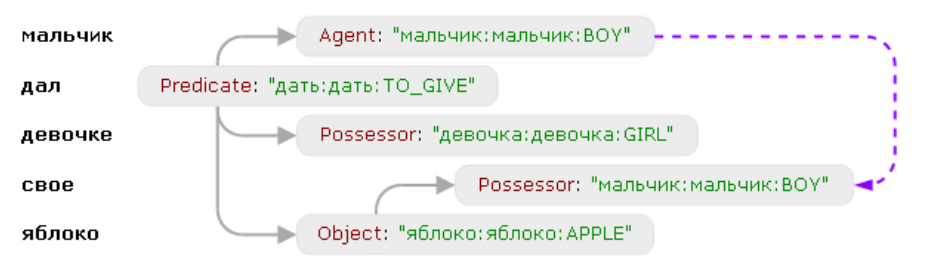
\includegraphics[width=0.9\linewidth]{images/compreno_syntax_with.png}
	\caption{Семантическое дерево, построенное системой Compreno, с дополнительными связями и подстановкой антецедента}
	\label{fig:compreno_syntax_with}
\end{figure}

Для реализации автоматизированного построения семантического дерева требуется корректная морфологическая и синтаксическая разметки, разрешение неоднозначности в которых требует, в свою очередь, наличия семантической разметки, что приводит к замкнутому кругу~\cite{Zaharov}.

В~\cite{bogdanov2014anaphora} также приведены общие сведения о способе разрешения кореференции между именами собственными и их кореферентами. Тем не менее, сделать какой-либо конкретный вывод о принципах работы данного механизма не представляется возможным.

\subsection{CogNIAC}

CogNIAC является алгоритмом разрешения анафоры в английском языке, построенным на системе правил~\cite{baldwin1997cogniac}. Для выполнения задачи алгоритму требуется следующая информация:
\begin{itemize}
	\item разделенный на предложения текст;
	\item выделенные именные группы, которые могут быть антецедентами;
	\item морфологическая разметка, в т.~ч. определение части речи, род, число;
	\item в одной из конфигураций~---~синтаксические деревья.
\end{itemize}

Основу алгоритма составляют 6 правил, перечисленные ниже.
\begin{enumerate}
	\item Уникальность в тексте: если существует единственный возможной антецедент в прочитанной части текста, то данный антецендент выбирается как истинный.
	\item Возвратность: истинным выбирается ближайший возможный антецедент в прочитанной части текста, если анафор является возвратным местоимением.
	\item Уникальность в текущем и предыдущем предложении: если существует единственный возможный антецедент в предыдущем и прочитанной части текущего предложения, то данный антецендент выбирается как истинный.
	\item Притяжательность: если анафор выражен притяжательным местоимением, и существует единственый антецедент в притяжательном падеже в предыдущем предложении, то данный антецедент выбирается как истинный.
	\item Уникальность в текущем предложении: если в прочитанной части текущего предложения существует единственный возможный антецедент, то данный антецедент выбирается как истинный.
	\item Уникальность подлежащего / местоимения в подлежащем: если подлежащее предыдущего предложения содержит единственный возможный антецедент и анафор является подлежащим текущего предложения, то такой антецедент выбирается истинным.
\end{enumerate}

Метод разрешения анафоры, используемый CogNIAC, работает следующим образом: местоимения обрабатываются слева направо, в порядке их появления в тексте; для каждого местоимения правила обрабатываются в порядке, в котором они приведены выше; для данного правила, если истинный антецедент найден, осуществляется соответствующая разметка и остальные правила не применяются к данному местоимению, иначе проверяется следующее правило; если ни одно ищ правил не подошло, анафора остается неразрешенной.

Данный алгоритм имеет некоторые фундаментальные ограничения. Одним из них является невозможность корректной обработки анафоры в предложениях вида~\cite{winograd1972understanding}: <<The city council refused to give the women a permit because they \{feared/advocated\} violence>>. Связано это с тем, что выбор верного антецедента здесь связан с употребляемым глаголом, в зависимости от которого, верным будет либо <<The city council>>, либо <<the women>>, однако, CogNIAC не учитывает значений глаголов в своих правилах. Другим ограничением является предположение о том, что антецедент находится в уже прочитанной части текста в пределах двух предложений от анафора. Однако, как отмечено в~\cite{mitkovStateOfArt}, антецедент может находиться на удалении до 17 предложений от анафора. Наконец, отмечается~\cite{baldwin1997cogniac}, что алгоритм не способен обработать множество антецедентов, имеющих общий анафор, например в отрывке: <<John called Mary. They went to a movie>>.

\subsection{Метод опорных векторов}

В~\cite{tolpegin2006algorithm} описано применение метода опорных векторов для разрешения анафоры местоимений третьего лица. В качестве входных данных были выбраны признаки текущего анафора и признаки гипотетических антецедентов, согласованных с анафором в роде и числа и встречавшихся ранее в тексте. В качестве признаков были выбраны:
\begin{itemize}
	\item число имен собственных между анафором и антецедентом;
	\item количество предложений, разделяющих анафору и антецедент;
	\item стоит ли антецедент в именительном падеже;
	\item является ли антецедент именем собственным;
	\item количество существительных и местоимений, расположенных в предложениях между рассматриваемыми анафором и антцедентом;
	\item совпадает ли падеж анафора и антецедента;
	\item статистическая информация о том, в каком сегменте предложения располагается антецедент~---~насколько близко к началу;
	\item статистическая информация о том, в каком сегменте предложения располагается анафор~---~насколько близко к началу;
	\item количество анафор, реферирующих с текущим антецедентом по данным ручной разметки, расположенных между анафорой и антецедентом;
	\item число глаголов в сегменте, содержащем антецедент;
	\item число причастий и деепричастий в сегменте, содержащем антецедент;
	\item число местоименных прилагательных и союзов в сегменте, содержащем антецедент;
	\item число существительных в именительном падеже в сегменте, содержащем антецедент;
	\item род, падеж и число анафоры и антецедента (в виде набора бинарных признаков). 
\end{itemize}

Исходный текст проходил предварительную морфологическую, синтаксическую и первичную семантическую разметку. Анафора местоимений третьего лица с существительными или другими местоимениями, в случае комплексной референции, была размечена вручную. 

Каждая пара анафора-гипотетический антецедент может быть отнесена к одному из двух классов, определяемых наличием или отсутствием референции. Утверждается~\cite{tolpegin2006algorithm}, что среди гипотетических антецедентов, предшествующих данному анафору обязательно найдется хотя бы один, связанный с ним референцией. Можно также полагать, что такой антецедент единственен, поскольку в силу транзитивности самого понятия анафоры, связность анафора со всему предшествующими антецедентами гарантируется. Для разрешения анафоры использовался следующий алгоритм:
\begin{enumerate}
	\item фиксируется очередной анафор и присваивается $n=1$;
	\item осуществляется переход к следующему $n$-ому гипотетическому антецеденту, согласованном в роде и числе, расположенному ранее в тексте, начиная с ближайшего к рассматриваемому анафору;
	\item для пары анафор-гипотетический антецедент запускается метод опорных векторов;
	\item выходные данные метода опорных векторов преобразуются в оценку связанности данной пары референтной связью с использованием сигмоиды;
	\item $n$ увеличивается на единицу. Если $n$ не превышает числа гипотетических антецедентов, осуществляется переход к шагу 2, иначе~---~к шагу 6;
	\item полученные оценки умножаются на релаксационные коэффициенты $r_i$, отражающие априорные знания о статистическом распределении анафор;
	\item рассматриваемый анафор связывается с $m$-ым антецедентом, где $m = argmax_n s_n$. Переход к шагу 1.  
\end{enumerate}

Поскольку чаще всего~\cite{tolpegin2006algorithm} анафор реферирует с ближайшим антецедентом, и вероятность референции падает с ростом $n$, коэффициенты релаксации определялись следующим образом:
\begin{equation}
	r_n = \Theta\frac{1}{N}+(1-\Theta)V_n,
\end{equation}
где коэффициент регуляризации $\Theta$ определялся с помощью кросс-валидации, а значение $N$ было принято равным 4.

Точность работы классификатора составила 62\%.